\newcommand{\TRESicmin}{1.85\xspace}
\newcommand{\TRESicmax}{3.10\xspace}
\newcommand{\TRESicNoveNoveMin}{1.62\xspace}
\newcommand{\TRESicNoveNoveMax}{3.33\xspace}
\newcommand{\TRESnZero}{26\xspace}


Foram retiradas 200 amostras, sem reposição, com tamanhos 4, 8, 16, 30 e 100, 
dentre os 4986 alunos que possuíam um valor definido para a variável Renda.
A população possuí média $\mu$ = ${\UMx}$ para a variável Renda, com desvio padrão $\sigma$ = ${\UMsd}$.
A \autoref{tab:q1} apresentam os valores da média e desvio padrão para cada tamanho
de amostra e seu respectivo valor esperado de desvio padrão.

\begin{table}[h]
\centering
\caption{Valores das médias amostrais para a variável \textit{Renda}}
\label{tab:q1}
\vspace{0.5em}
\begin{tabular}{l r r r}
	\toprule
	\textbf{\specialcell{c}{Tamanho da\\Amostra}} & \textbf{Média} & \textbf{\specialcell{c}{Desvio\\Padrão}} & \textbf{$\frac{\sigma}{\sqrt{n}}$}\\
	\midrule
	$4$       & ${\UMxQuatro}$   & ${\UMsdQuatro}$   & ${\UMsdeQuatro}$   \\
	$8$       & ${\UMxOito}$   & ${\UMsdOito}$   & ${\UMsdeOito}$   \\
	$16$      & ${\UMxDezesseis}$  & ${\UMsdDezesseis}$  & ${\UMsdeDezesseis}$  \\
	$30$      & ${\UMxTrinta}$  & ${\UMsdTrinta}$  & ${\UMsdeTrinta}$  \\
	$100$     & ${\UMxCem}$ & ${\UMsdCem}$ & ${\UMsdeCem}$ \\
	\bottomrule
\end{tabular}
\end{table}

\subsection{Valor esperado da média amostral}
Na \autoref{tab:q1} é possível observar que a medida que se aumenta o tamanho da amostra o valor da média amostral fica cada vez mais próximo do valor da média populacional, que é de ${\UMx}$.


\subsection{Valor esperado do desvio padrão da média amostral}
Conforme indicado na \autoref{tab:q1}, os valores de desvio padrão das amostras ficam mais próximos dos valores de $\frac{\sigma}{\sqrt{n}}$ à medida que se aumenta o tamanho das amostras.

\subsection{Distribuição amostral da média}
Conforme indicado nas Figuras 1 à 5, a medida que se aumenta o tamanho das amostras,
a distribuição amostral da média se torna similar à uma distribuição normal.

\begin{figure}[h]
\begin{minipage}{0.50\textwidth}
	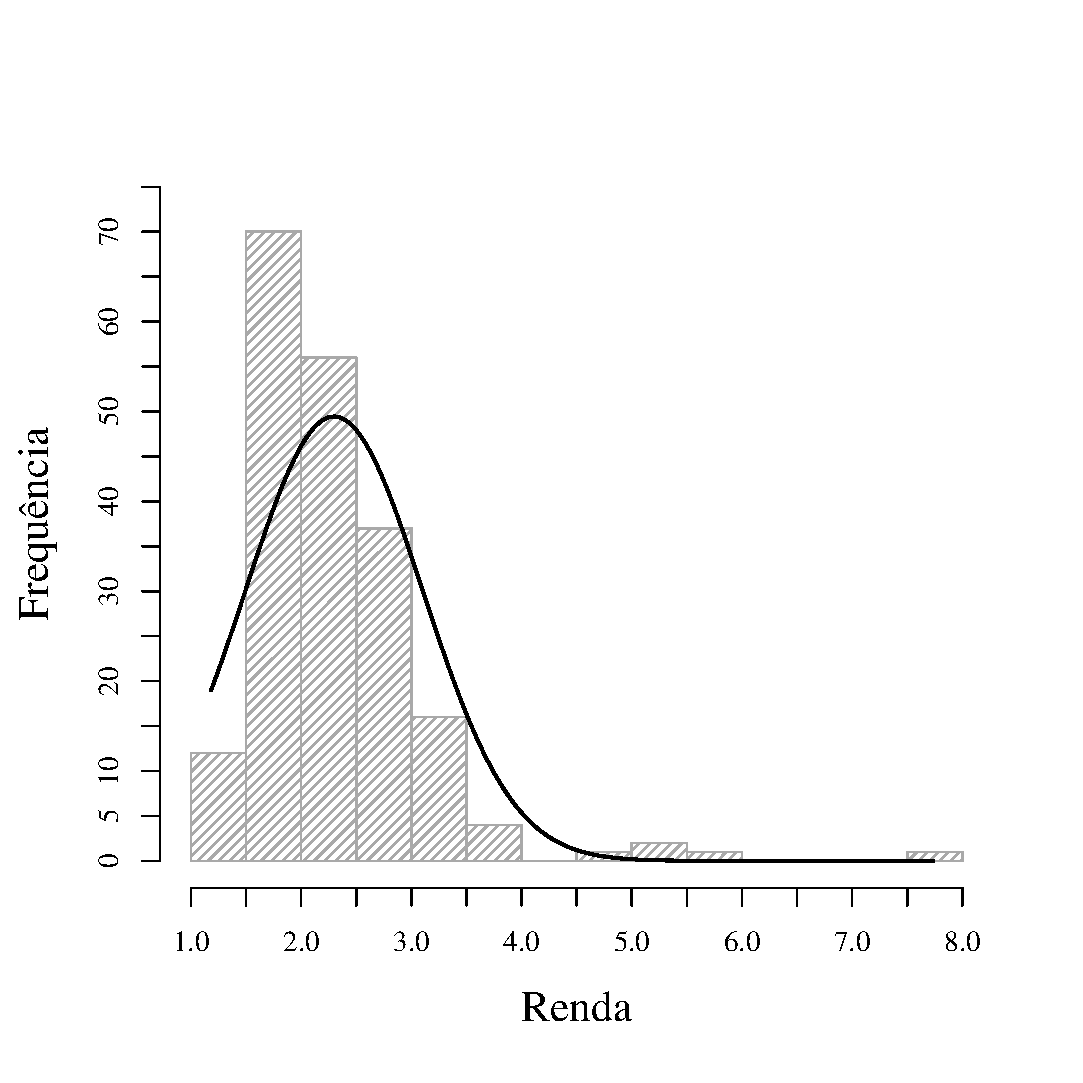
\includegraphics[width=\linewidth]{plots/histogram_renda_n4.eps}
	\caption{Distribuição amostral da média para amostras de tamanho 4}
	\label{fig:m4}
\end{minipage}
\begin{minipage}{0.50\textwidth}
	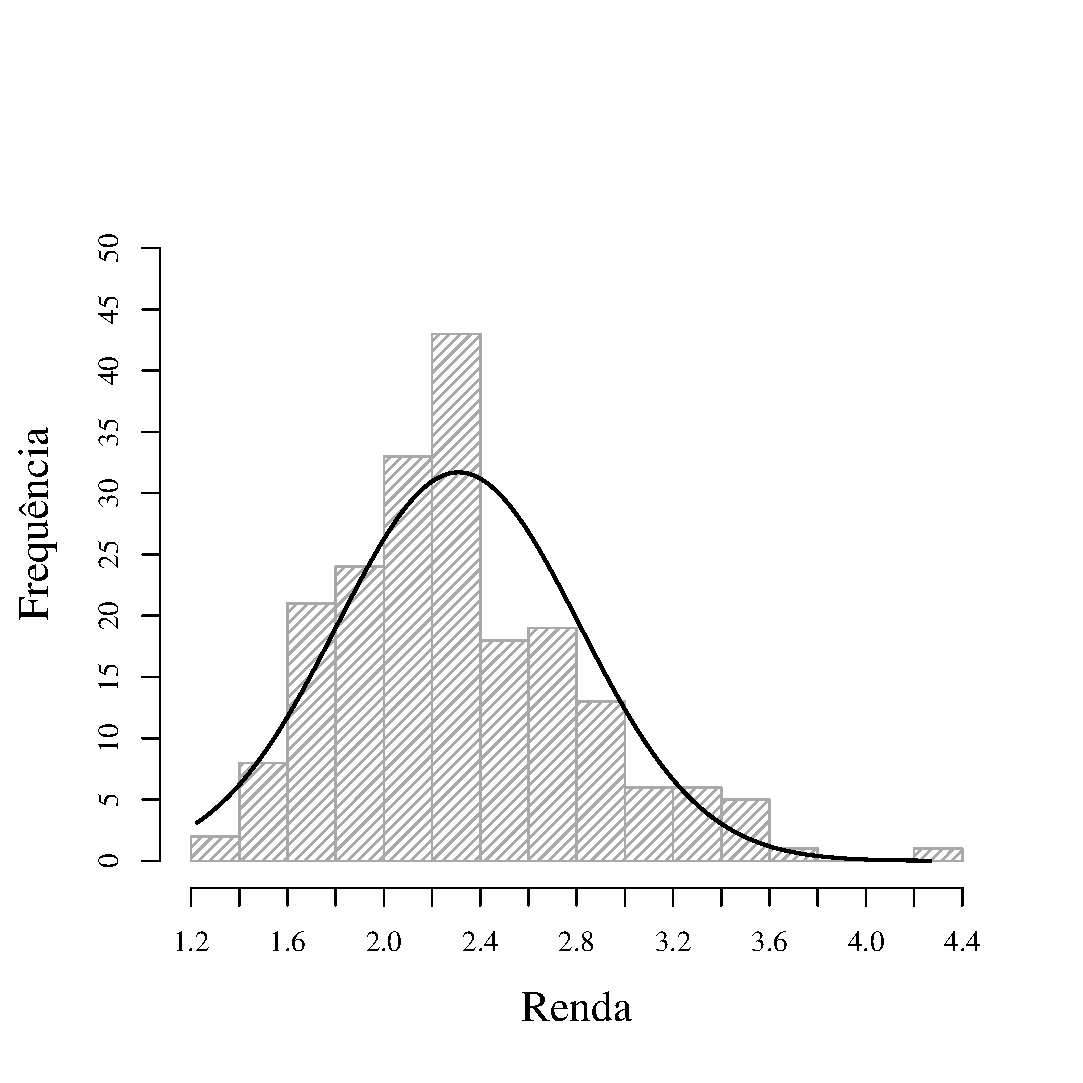
\includegraphics[width=\linewidth]{plots/histogram_renda_n8.eps}
	\caption{Distribuição amostral da média para amostras de tamanho 8}
	\label{fig:m8}
\end{minipage}
\end{figure}

\begin{figure}[h]
\begin{minipage}{0.50\textwidth}
	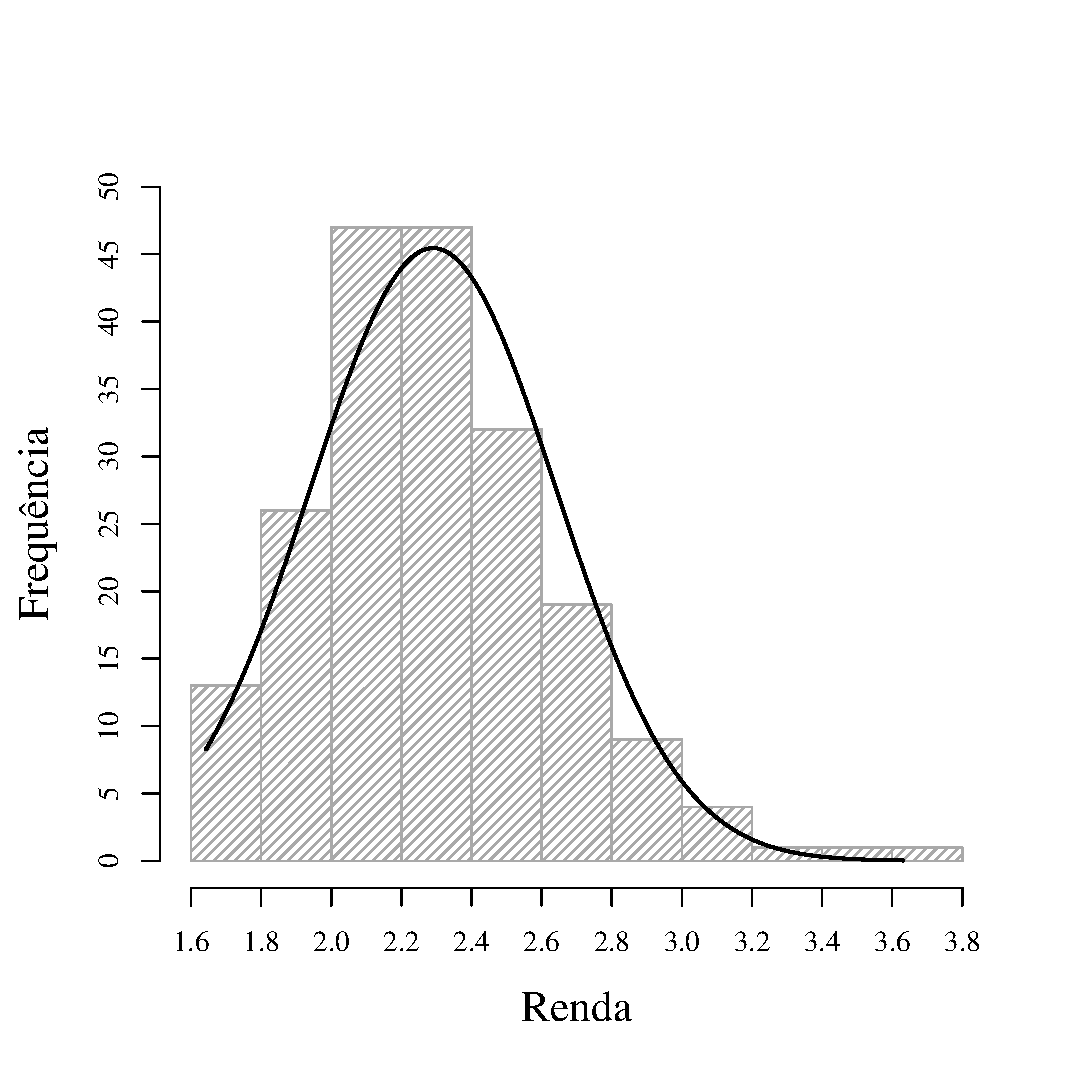
\includegraphics[width=\linewidth]{plots/histogram_renda_n16.eps}
	\caption{Distribuição amostral da média para amostras de tamanho 16}
	\label{fig:m16}
\end{minipage}
\begin{minipage}{0.50\textwidth}
	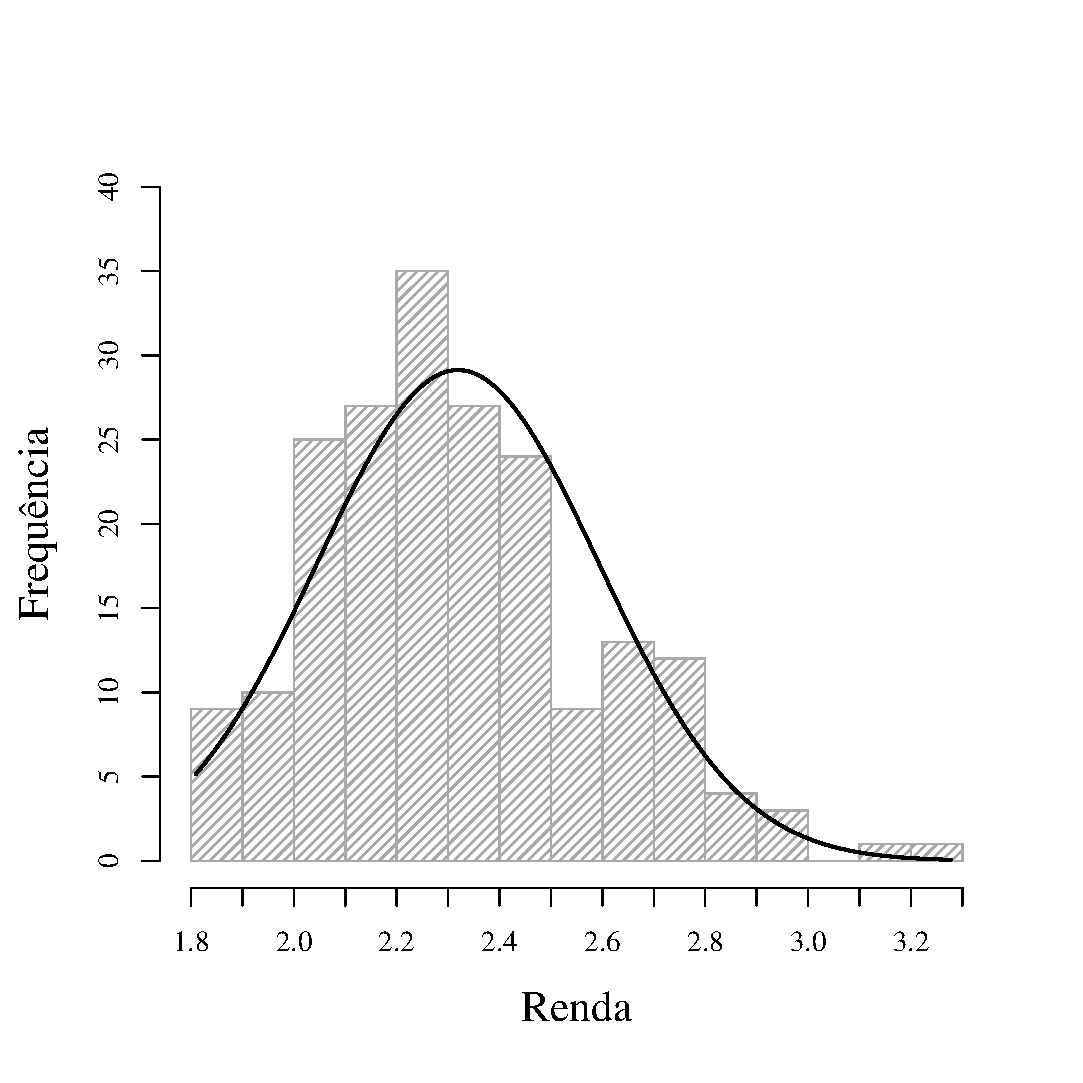
\includegraphics[width=\linewidth]{plots/histogram_renda_n30.eps}
	\caption{Distribuição amostral da média para amostras de tamanho 30}
	\label{fig:m30}
\end{minipage}
\end{figure}

\begin{figure}[h]
\centering
	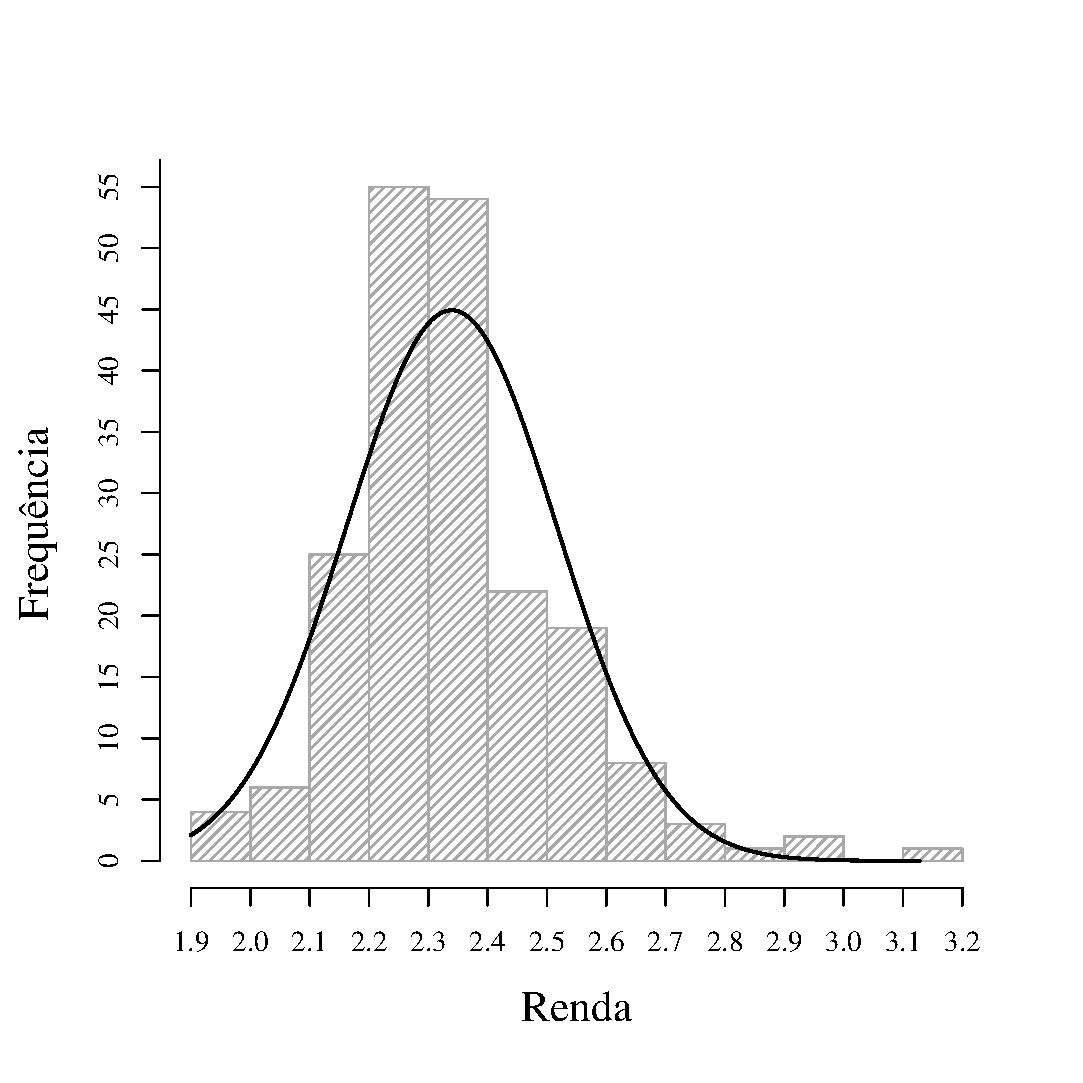
\includegraphics[width=0.50\textwidth]{plots/histogram_renda_n100.eps}
	\caption{Distribuição amostral da média para amostras de tamanho 100}
	\label{fig:m100}
\end{figure}

\FloatBarrier
